% Figure 6 — secondary Q8(K1) extension.
% Asset generated by scripts/publication_figures/fig06_q8.py
\begin{figure}[tb]
  \centering
  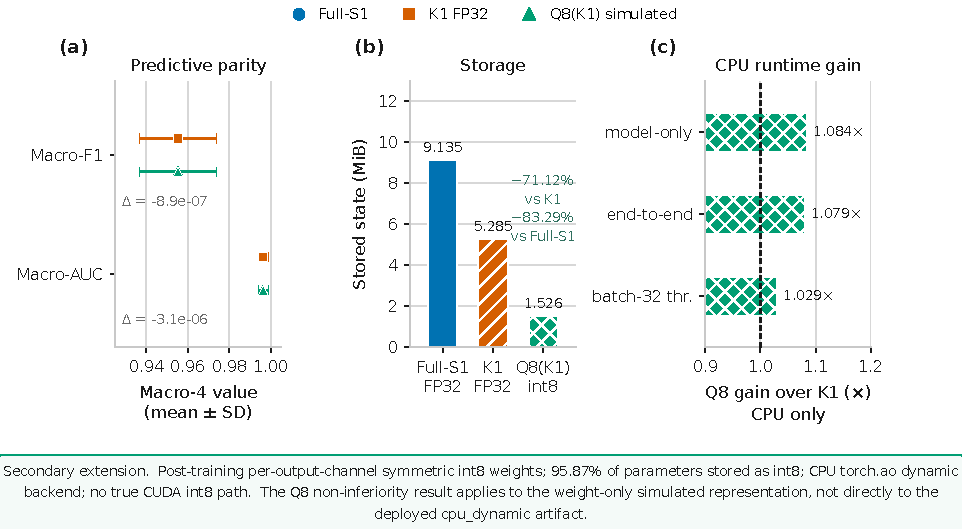
\includegraphics[width=\textwidth]{figures/fig06_q8_extension.pdf}
  \caption{Secondary Q8(K1) deployment extension. (a) The weight-only simulated
  Q8 representation matches K1 FP32 on both Macro-4 endpoints, with paired mean
  differences of order $10^{-6}$ or smaller. (b) Stored state-dictionary size
  for the representative fold--seed cell. (c) CPU runtime gain of Q8 over K1,
  measured within the Q8 benchmark, against a parity line. The predictive
  result applies to the simulated weight-only representation and does not
  transfer automatically to the deployed \texttt{cpu\_dynamic} artifact; no GPU
  int8 execution path exists on the preserved stack.}
  \label{fig:q8}
\end{figure}
